\chapter{Image Compression}\label{Ch:ImageProcessing}

GPUs have become increasingly common in machine learning due
to their rapid matrix multiplication. While we had access to
GPUs, the on-board memory was not sufficient to store the
images in the experience replay memory. Consequently, 
host-to-device transfer must occur to properly store all
images. In an effort to reduce the required memory, we
converted the eight-bit grayscale representation of 
images to binary images, reducing the memory consumption by
a factor of eight. The benefits of this compression
are twofold: foremost, we reduce the memory required,  and the 
agent learns to follow the road more closely. The latter is
discussed further in the next few sections.

\section{Edge Detection}
Upon completing a racetrack, we found that the car would not continue to drive on the road. This
suggested the agent learned to follow the tiles on the road; in their absence, the agent did 
not know to continue on the road to collect the missed tiles. While pursuing
tiles is a reasonable strategy for maximizing rewards in the game, this behavior is
at least detrimental in seeking missed tiles and at worst adverse in the context of real-life driving. 
To mend this, we altered the representation of the images fed into the network 
so that tiles were not visible to the agent.
An example of the altered image is given in Figure \ref{fig:canny_example}.

\begin{figure}[h]
\centering
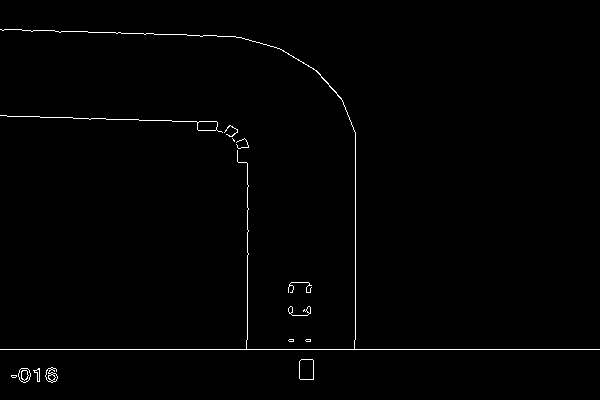
\includegraphics[width=0.6\textwidth]{Graphics/standard_gray_1_canny.png}
\caption{Edge detection compression}
\label{fig:canny_example}
\end{figure}

With this compression method, the
agent no longer sees tiles and must learn to stay on the road to receive rewards.
The method in question is a form of edge detection known as the Canny edge 
detection algorithm \cite{canny}. The next few sections provide an overview
of the Canny algorithm followed by a discussion of the 
performance of our
algorithm with this updated representation.

\newpage
\subsection{Canny Edge Detection}
The Canny algorithm consists of five main steps:

\begin{enumerate}[1.]
\item{Conversion from RGB to grayscale.}
\item{Noise suppression.}
\item{Gradient approximation.}
\item{Non-maximum edge suppression}
\item{Hysteresis thresholding}
\end{enumerate}

Each step is discussed in detail in the next few sections.

\subsection{RGB to Grayscale}
Several methods exist for converting a
red-green-blue (RGB) color image to grayscale, though
all reduce to taking a weighted average of each color channel. We used the 
conversion in Equation (\ref{eq:rgb2gray}), where $R,G,B$ represent the
red, green, and blue color channels (respectively) of the RGB image. 

\begin{align}\label{eq:rgb2gray}
Gray = .299R + .587G + .114B
\end{align}

An example of a grayscale conversion using Equation (\ref{eq:rgb2gray}) is given in 
Figure \ref{fig:rgb_to_grayscale}.

\begin{figure}[h]
\centering
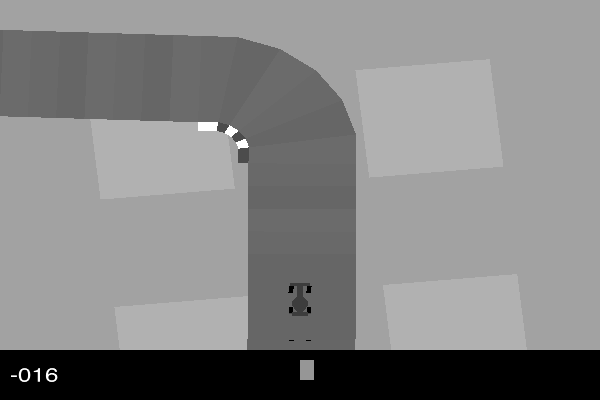
\includegraphics[width=0.6\textwidth]{Graphics/standard_gray_1.png}
\caption{Grayscale image representation}
\label{fig:rgb_to_grayscale}
\end{figure}

\subsection{Noise Suppression}
Edge detection is typically applied to images captured by digital cameras
and inherently exhibit some noise. For our purposes, `noise' refers to
regions in the image that are not crucial in the agent's learning how
to navigate the tracks. Such regions are the tiles and grass squares
visible in Figure \ref{fig:rgb_to_grayscale}.

A common technique used to 
suppress noise is image smoothing where pixel values are replaced
by a weighted average of its neighbors. This weighted average computation
is typically performed via convolution. Given two continuous functions 
$f,g$ with bounded support $[0, \infty)$, the convolution of $f$ and $g$
gives a third function and is defined as

\begin{align}\label{eq:cont_conv}
(f*g)(t) &= \int_0^t f(\tau)g(t-\tau)d\tau.
\end{align}

For discrete functions, the convolution is given by

\begin{align}\label{eq:disc_conv}
(f*g)(t) &= \sum_{\tau=0}^t f(\tau)g(t-\tau).
\end{align}

\par
To be more precise, let $f$ above denote the grayscale image obtained
using Equation (\ref{eq:rgb2gray}). $g$ will then be a two-dimensional matrix,
called a kernel, that determines how much weight to give to neighboring
pixels. We used the $3\times 3$ Gaussian kernel given below

\begin{align*}
g &=
\begin{bmatrix}
0.0751 & 0.1238 & 0.0751 \\
0.1238 & 0.2042 & 0.1238 \\
0.0751 & 0.1238 & 0.0751
\end{bmatrix}
\end{align*}

which can be found by taking the matrix below and dividing so that the
matrix entries sum to 1; $h$ here refers to the 
bivariate Gaussian density 
$\mathcal{N}\left([0,0],\begin{bmatrix} 1 & 0  0 & 1 \end{bmatrix}\right)$.

\begin{align*}
\begin{bmatrix}
h(-1,-1) & h(0,-1) & h(1,-1) \\
h(-1,0) & h(0,0) & h(1,0) \\
h(-1, 1) & h(0, 1) & h(1,1)
\end{bmatrix}.
\end{align*}

Let $h$ now be the output of convolving the image $f$ with kernel $g$, then
$h(m,n$) is given by

\begin{align}\label{eq:img_conv}
h(m,n) &= \sum_{k=-1}^{1} \sum_{l=-1}^{1} f(m-k,n-l)g(k,l)
\end{align}

where $g$ is indexed such that the top left entry is entry $(-1,-1)$
and its bottom right entry is $(1,1)$. $h$ now represents the smoothed image;
this operation is typically referred to as a Gaussian blur. 

\subsection{Gradient approximation}
For our purposes, an edge refers to a change in pixel intensity. Change in 
functions is typically quantified by differentiation; the same applies to
images.
Having smoothed the image using Equation \ref{eq:img_conv}, edges are identified
by computing this image's gradient. Letting $f$ be a differentiable function,
its derivative at $x$, $f'(x)$, is defined as

\begin{align}\label{eq:derivative_def}
f'(x) &= \lim_{h \to 0} \frac{f(x+h) - f(x)}{h}.
\end{align}

For a small enough $h$, $f'(x)$ can be approximated using the forward 
difference approximation in Equation (\ref{eq:finite_diff_forward}).

\begin{align}\label{eq:finite_diff_forward}
f'(x) \approx \frac{f(x+h) - f(x)}{h}
\end{align}

For images, a more accurate derivative approximation is the central difference
defined in Equation (\ref{eq:finite_diff_central}).

\begin{align}\label{eq:finite_diff_central}
f'(x) \approx \frac{f(x+.5h) - f(x-.5h)}{h}
\end{align}

An image is two-dimensional and hence has derivatives along two axes, which
we call $x$ and $y$.
Thus, given a signal such as that in Table \ref{table:1dSignal}--which can be
interpreted as the row of an image--it can be differentiated using Equation
(\ref{eq:finite_diff_central}). 

\begin{table}
\centering
\begin{tabular}{|c|c|c|c|c|}
\hline 
40 & 40 & 200 & 240 & 100 \\
\hline
\end{tabular}
\caption{1-dimensional signal}
\label{table:1dSignal}
\end{table}

For example, to estimate the derivative
of the signal at the third pixel value of 200, we compute
$\frac{240-40}{2} = 100$. 

Padding the image with zeros allows us to perform the operation above to
every pixel in the signal. Up to scaling by a constant, this operation is computationally equivalent to convolving the signal with the
kernel $[-1, 0, 1]$. Thus to obtain the gradient along the $x$ direction
of an image, we simply need to convolve it with the kernel $[-1, 0 ,1]$. 
This operation outputs a grayscale image with edges most prominent along
the original image's $x$ direction; however, this also introduces `false 
edges'--edges that may not necessarily be edges of interest. To remedy
this, we blur the outputted image with a smoothing filter. In particular,
we will convolve the gradient approximation with the kernel 
$[1, 2, 1]^T$. We smooth along the y-axis so that false edges parallel
to the x-axis are averaged. Thus, to obtain the gradient along the
x-direction of the smoothed image, $h$, given by Equation (\ref{eq:img_conv}), we 
compute

\begin{align}\label{eq:grad_x_1}
I_x &= h * 
\begin{bmatrix}
-1 & 0 & 1
\end{bmatrix} *
\begin{bmatrix}
1  2  1
\end{bmatrix}.
\end{align}

The convolution operation is associative, allowing us to first convolve
the filters in Equation (\ref{eq:grad_x_1}) to obtain

\begin{align}\label{eq:grad_x_2}
I_x &= h * 
\begin{bmatrix}
-1 & 0 & 1 \\
-2 & 0 & 2 \\
-1 & 0 & 1
\end{bmatrix}
\end{align}

where the filter on the right of Equation (\ref{eq:grad_x_2}) is called the Sobel 
filter. In literature, the filter above may be presented as having the
negative values on the rightmost column and the positive values on the
leftmost column; we prefer our representation as it illustrates how the
kernel arises. Moreover, the sign of the kernel is not imperative as
we are interested in magnitudes. 

We can similarly obtain the gradient along the y-axis by convolving with
the transpose of the Sobel kernel given in Equation (\ref{eq:grad_x_2}):

\begin{align}\label{eq:grad_y_1}
I_y &= h * 
\begin{bmatrix}
-1 & -2 & -1 \\
0 & 0 & 0 \\
1 & 2 & 1
\end{bmatrix}.
\end{align}

Having obtained the gradients along the x and y axes, the magnitude of
the gradient, $I$, can be obtained by computing

\begin{align}\label{eq:gradient_mag}
I &= \sqrt{I_x^2 + I_y^2}.
\end{align}

Similarly, the direction of the gradient, $\theta$, can be obtained by
computing

\begin{align}\label{eq:gradient_direc}
\theta &= \textrm{arctan}\left(\frac{I_y}{I_x}\right).
\end{align}

At this juncture, $I$ in Equation (\ref{eq:gradient_mag}) represents the edges of
the image, though it contains false edges. The next two sections discuss
methods to suppress these edges using $\theta$ and hysteresis 
thresholding.

\subsection{Non-Maximum Edge Suppression}
By smoothing the original grayscale image, we have changed the values
of the pixels such that we will ultimately be able to remove them in
the final step of the Canny algorithm. At this stage, it is possible
that the unwanted edges are still present in $I$. Indeed, this is 
corroborated by visualizing $I$ in Figure \ref{fig:thick_edges_example}
where the tile and grass edges are clearly visible. These will be
removed in the next step of the Canny algorithm, but this image
reveals another potential issue: the edges are very thick. This
step of the edge detection algorithm aims to thin these edges via
a method known as non-maximum edge suppression.

\begin{figure}[h]
\centering
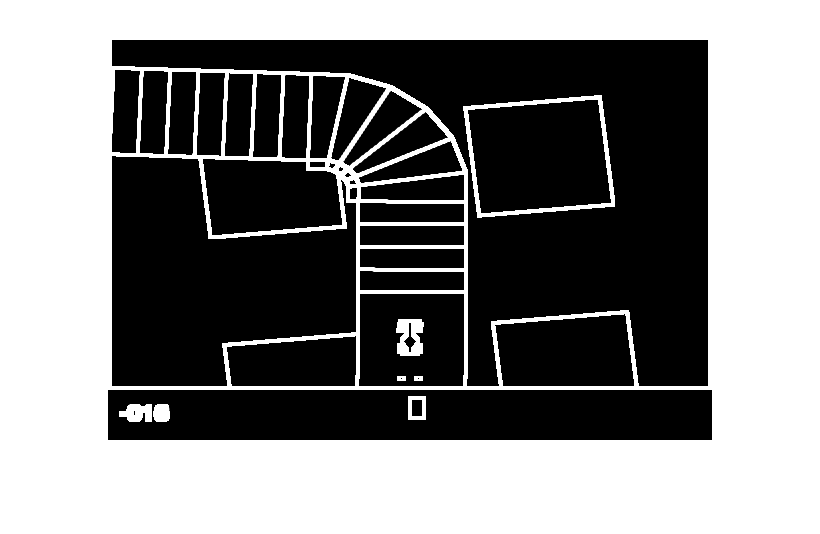
\includegraphics[width=0.6\textwidth]{Graphics/thick_edges_example.png}
\caption{Thick edges}
\label{fig:thick_edges_example}
\end{figure}

This technique goes through every pixel in $I$ and compares the pixel
value to the value of its neighbors; if the pixel value is larger
than those of its neighbors, it is kept, otherwise it is set to 0. 
If $(i,j)$ represents the pixel in question, its `neighbors' are defined
to be the pixels parallel to the direction of $(i,j)$ where the
direction is given by the gradient direction at $(i,j)$--that is, 
$\theta(i,j)$. 

\par
Images are discrete objects and each pixel is surrounded by eight
potentially neighboring pixels. Thus, the direction of a pixel's gradient
must be discretized into eight possible directions. As such, every entry
in $\theta$ will be binned into eight possible directions: north to south, 
south to north, east to west, west to east, southwest to northeast, 
northeast to southwest, northwest to southeast, and southeast to 
northwest. A diagram illustrating these directions is given in 
Figure \ref{fig:disc_grad_dir}. 

\begin{figure}
\centering
\begin{subfigure}{.5\textwidth}
  \centering
  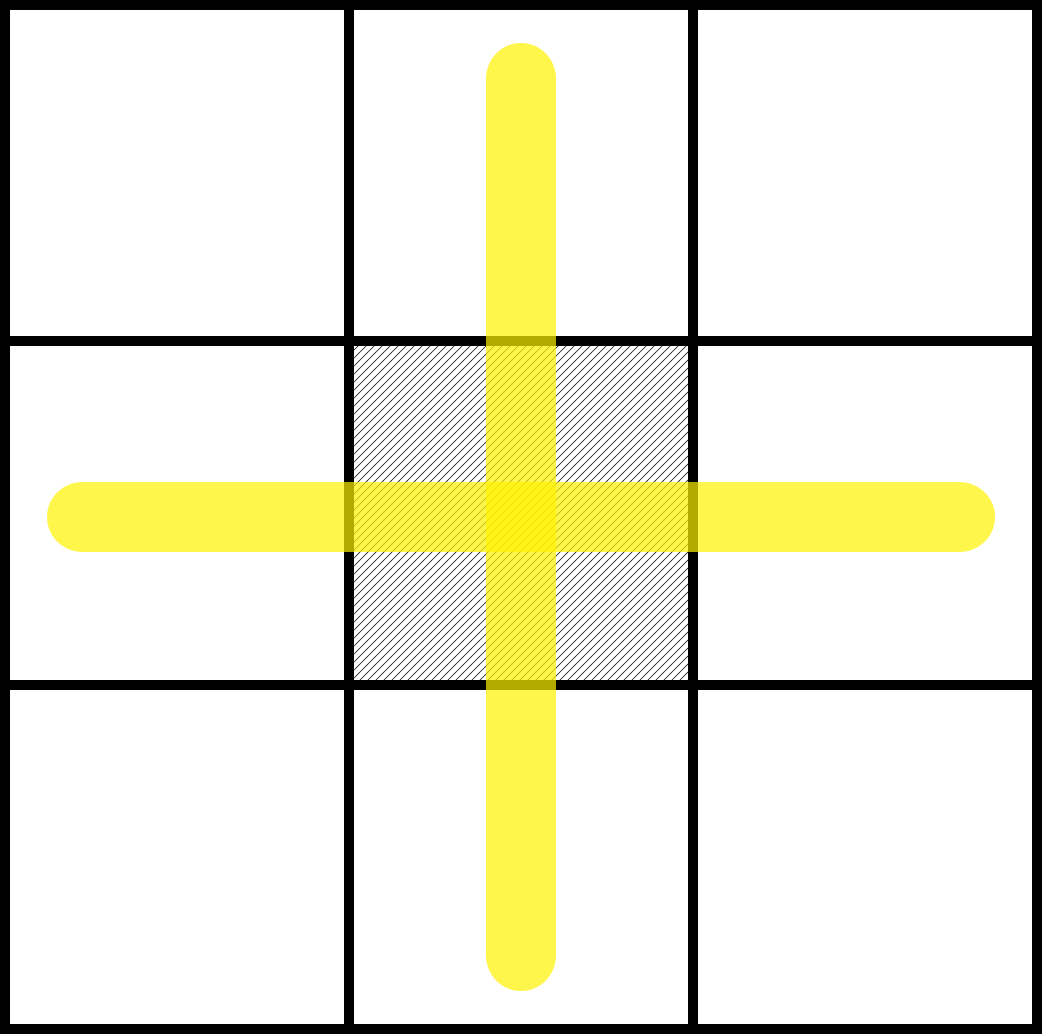
\includegraphics[width=.4\linewidth]{Graphics/disc_grad_dir_cross.png}
  \caption{N to S, W to E}
  \label{fig:disc_grad_dir_cross}
\end{subfigure}%
\begin{subfigure}{.5\textwidth}
  \centering
  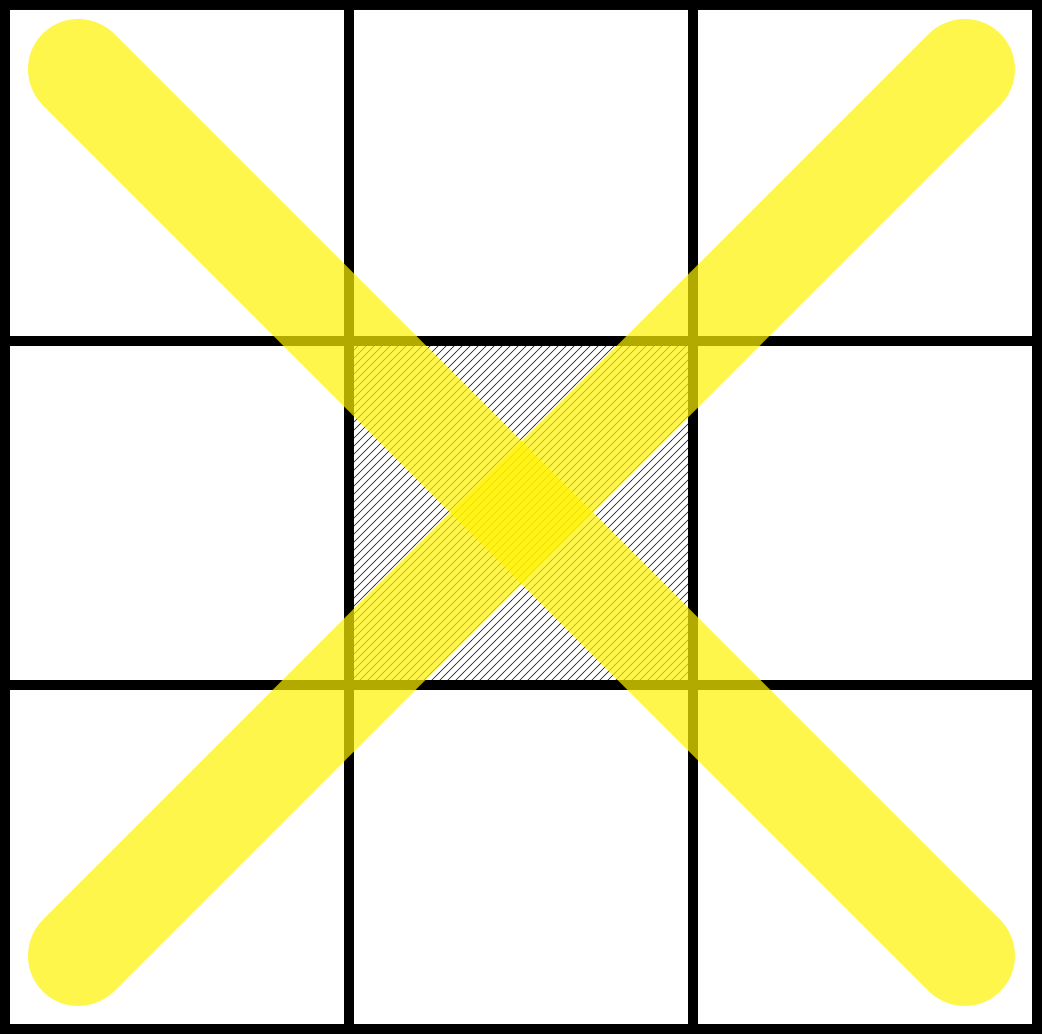
\includegraphics[width=.4\linewidth]{Graphics/disc_grad_dir_diag.png}
  \caption{NW to SE, SW to NE}
  \label{fig:disc_grad_dir_diag}
\end{subfigure}
\caption{Discretized gradient directions}
\label{fig:disc_grad_dir}
\end{figure}

This diagram depicts a clear redundancy: directions can be discretized
into four bins. As such, gradient directions will be classified as one of:
north to south, west to east, northwest to southeast, and southwest to 
northeast. The discretization is performed as shown in Table 
\ref{table:grad_discretization}, where the left column is the value
of $\theta$ in degrees and the right column is the corresponding bin;
the notation $(a,b)$ denotes the set of numbers in the range from $a$
to $b$. 

\begin{table}
\centering
\begin{tabular}{c|c}
Angle & Bin \\
\hline
(0, 22.5) $\cup$ (157.5, 202.5) $\cup$ (337.5, 360) & W to E \\
(22.5, 67.5) $\cup$ (202.5, 247.5) & SW to NE \\
(67.5, 112.5) $\cup$ (247.5, 292.5) & N to S \\
(112.5, 157.5) $\cup$ (292.5, 337.5) & NW to SE
\end{tabular}
\caption{Gradient direction binning}
\label{table:grad_discretization}
\end{table}

Once the gradient directions have been discretized, every pixel in
$I$ is compared to its neighbors. The neighbors of a pixel are determined
by the direction of its gradient. The neighbors for every gradient
direction is given in Figures \ref{fig:disc_grad_dir_neighbors_1}
and \ref{fig:disc_grad_dir_neighbors_2}. 

\begin{figure}[h!]
\centering
\begin{subfigure}{.5\textwidth}
  \centering
  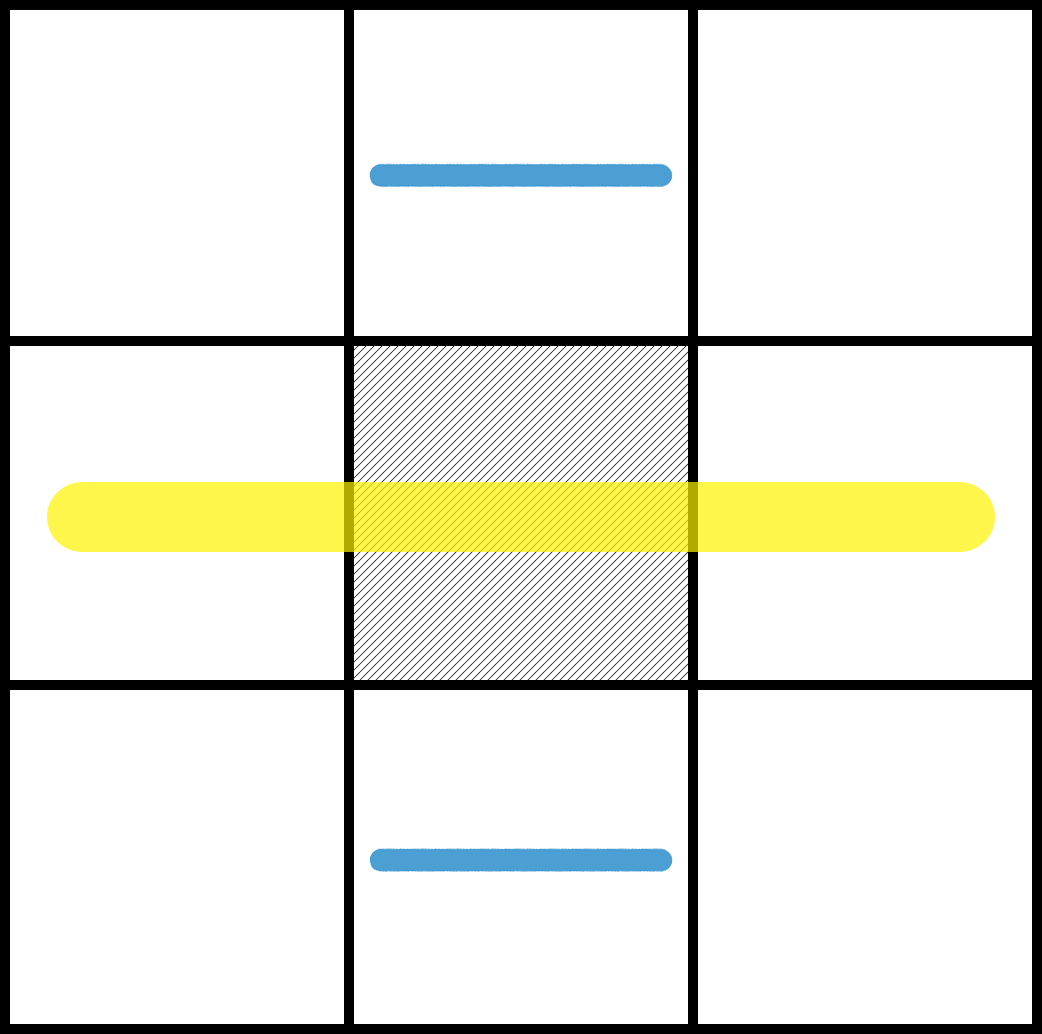
\includegraphics[width=.4\linewidth]{Graphics/disc_grad_dir_neighb_horizontal.png}
  \caption{W to E neighbors}
  \label{fig:disc_grad_dir_horiz}
\end{subfigure}%
\begin{subfigure}{.5\textwidth}
  \centering
  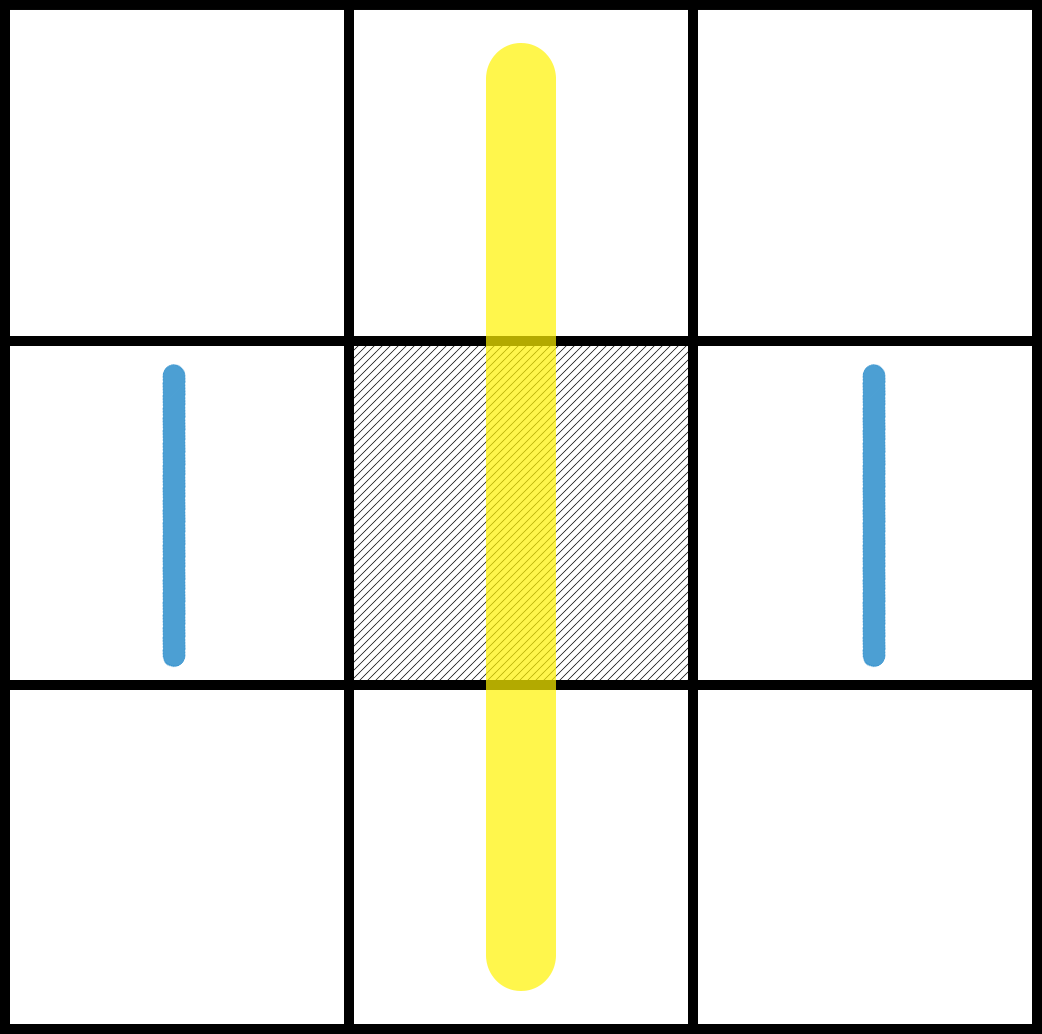
\includegraphics[width=.4\linewidth]{Graphics/disc_grad_dir_neighb_vertical.png}
  \caption{N to S neighbors}
  \label{fig:disc_grad_dir_vert}
\end{subfigure}
\caption{Discretized gradient directions}
\label{fig:disc_grad_dir_neighbors_1}
\end{figure}

\begin{figure}[h!]
\centering
\begin{subfigure}{.5\textwidth}
  \centering
  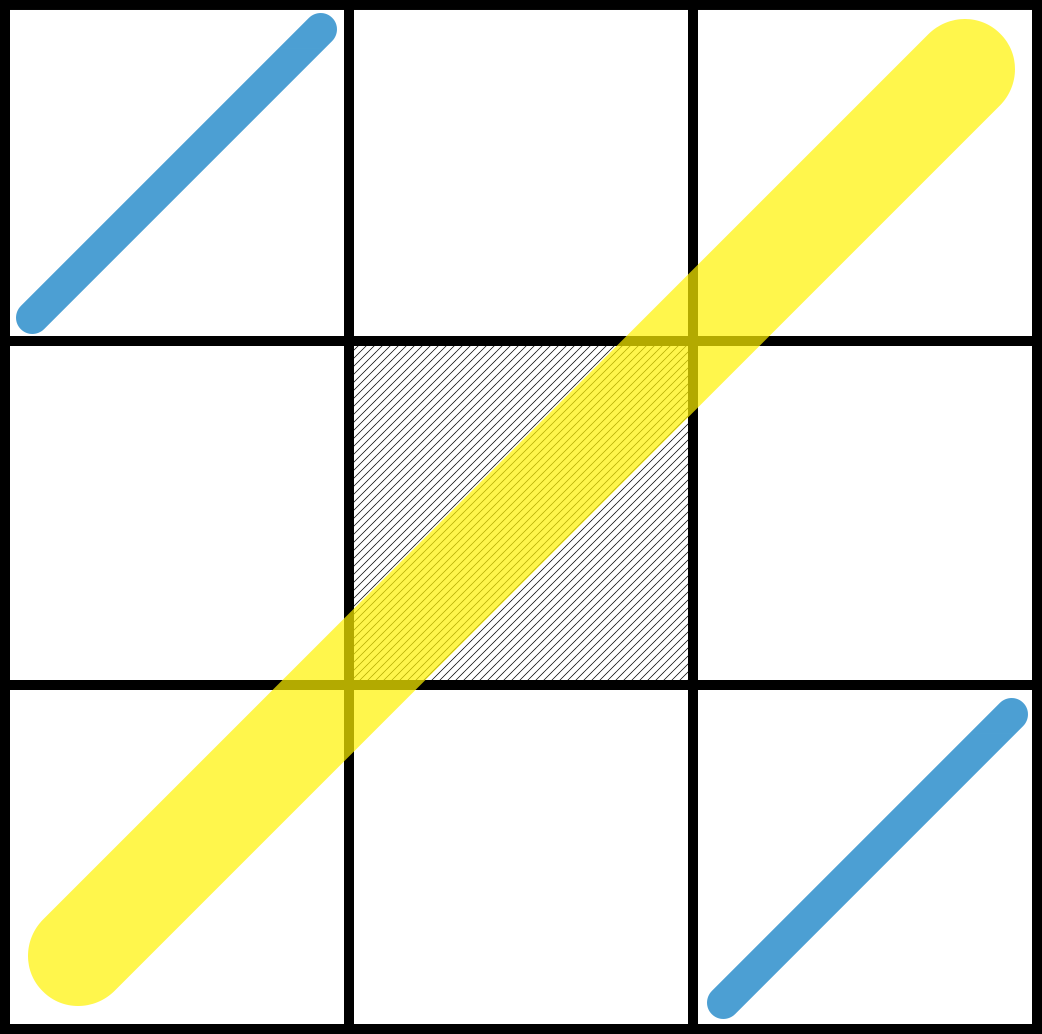
\includegraphics[width=.4\linewidth]{Graphics/disc_grad_dir_diag_1.png}
  \caption{SW to NE neighbors}
  \label{fig:disc_grad_dir_diag_1}
\end{subfigure}%
\begin{subfigure}{.5\textwidth}
  \centering
  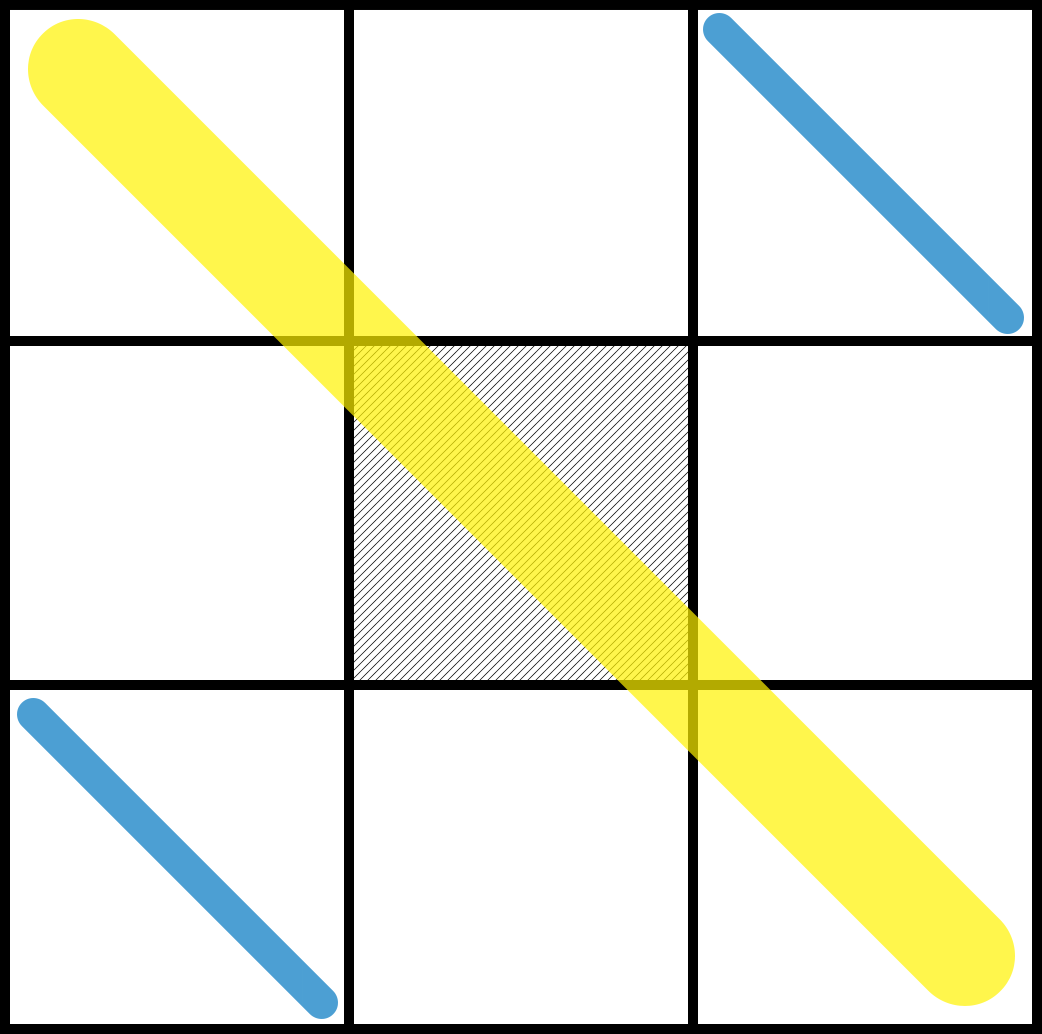
\includegraphics[width=.4\linewidth]{Graphics/disc_grad_dir_diag_2.png}
  \caption{NW to SE neighbors}
  \label{fig:disc_grad_dir_diag_2}
\end{subfigure}
\caption{Discretized gradient directions}
\label{fig:disc_grad_dir_neighbors_2}
\end{figure}

For example, if pixel $(i,j)$ has a gradient direction of SW to NE
as in Figure \ref{fig:disc_grad_dir_diag_1}, then the
neighbors of $(i,j)$ are pixels $(i-1,j-1)$ and $(i+1,j+1)$. We then
compare the value of pixel $(i,j)$ to its neighbors and set it to zero
if its value is less than those of its neighbors, otherwise its value
remains the same. 

After performing the operation outlined above, we obtain an image
similar to that in Figure \ref{fig:thick_edges_example}, though
now the edges have been thinned as shown in Figure 
\ref{fig:thin_edges_example}.

\begin{figure}[h!]
\centering
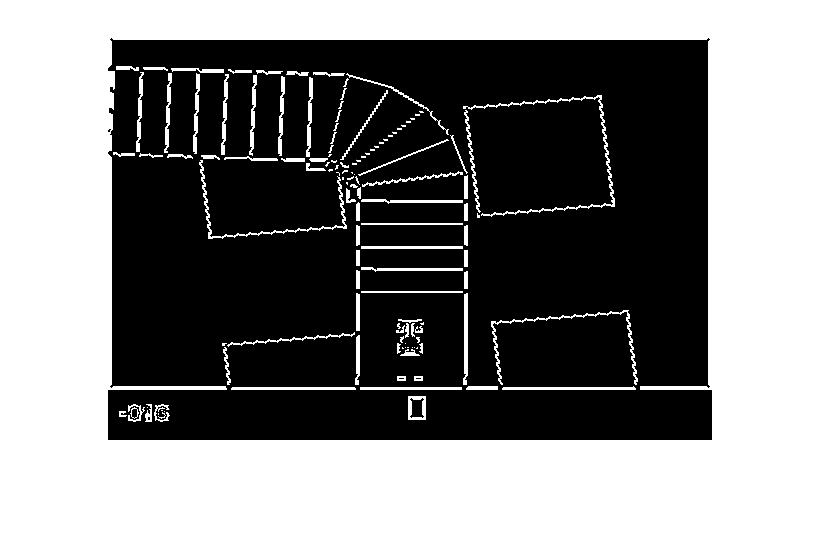
\includegraphics[width=0.6\textwidth]{Graphics/thinned_edges_example.png}
\caption{Thin edges}
\label{fig:thin_edges_example}
\end{figure}

\subsection{Hysteresis Thresholding}
After performing non-maximum edge suppression via the procedure outlined
above, the final step of the Canny edge detection algorithm is to remove
edges that are deemed insignificant. More precisely, we will introduce
two parameters $a,b \in \{0,1,2,\ldots, 255\}$ $a > b$ known as
thresholds. Then, every pixel in the thinned image will be compared to 
these thresholds: values less than $b$ will be discarded (set to zero), 
and values greater than $a$ will be kept (set to one). Values 
between $a$ and $b$ will be kept only if the pixel is connected to
an edge with a pixel value greater than $a$. More precisely, 
if the value of pixel $(i,j)$ is between $a$ and $b$, we will look
at its neighbors (as determined by the gradient direction) and 
set the value of pixel $(i,j)$ to one if one of its neighbors has
a value greater than $a$, otherwise it will be set to zero.

For our algorithm we used the thresholds $a = 150$ and $b=250$. 
Applying hysteresis thresholding to Figure \ref{fig:thin_edges_example}
yields the image in Figure \ref{fig:canny_example}.

\subsection{Edge Detection Performance}
In writing, feeding the output of the compressed edge detected image
offers several benefits: the agent learns to stay on the road and the
required memory decreases by a factor of eight. However, it is 
important to verify these claims. The orange curve in Figure 
\ref{fig:aveQ_edge} plots the average Q-function of our algorithm when 
the images fed are those passed through the edge detection algorithm; the
blue line depicts the average Q-function when the images are simply 
grayscale images. In particular, both models were trained on three
fixed tracks and tested on random ones. Both methods converge to similar 
values, suggesting the algorithm retains its generalizability. Moreover,
the orange curve in Figure \ref{fig:test_edge} depicts the average
training score for the edge detection algorithm as compared to the
grayscale algorithm (in blue); there is no evidence suggesting the
performance of the algorithm is compromised. 


In short, by first passing the images output by the environment through
an edge detection compression, we are able to reduce the amount of 
memory required for training, and retain the performance obtained 
without compressing the image. 

\begin{figure}[]
\centering
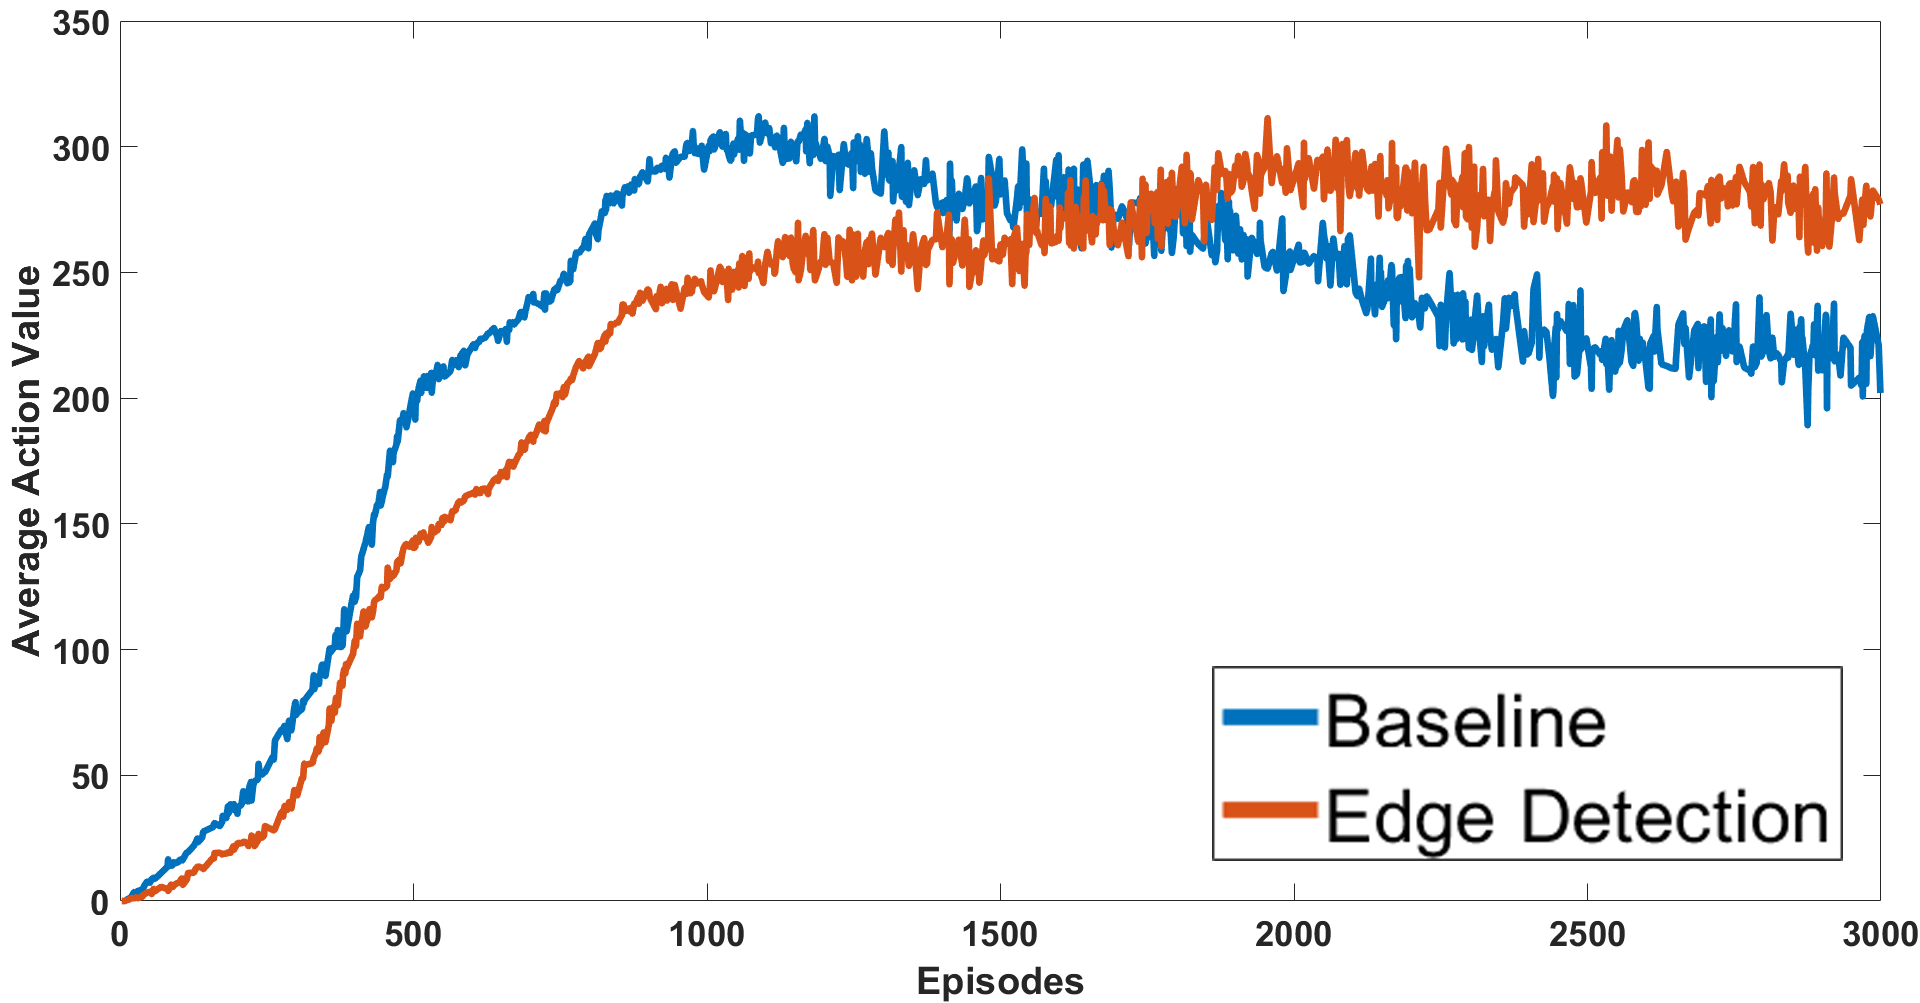
\includegraphics[width=.6\linewidth]{Graphics/edge_perf_q_large.png}
\caption{Average Q-value for edge detection}
\label{fig:aveQ_edge}
\end{figure}

\begin{figure}[]
\centering
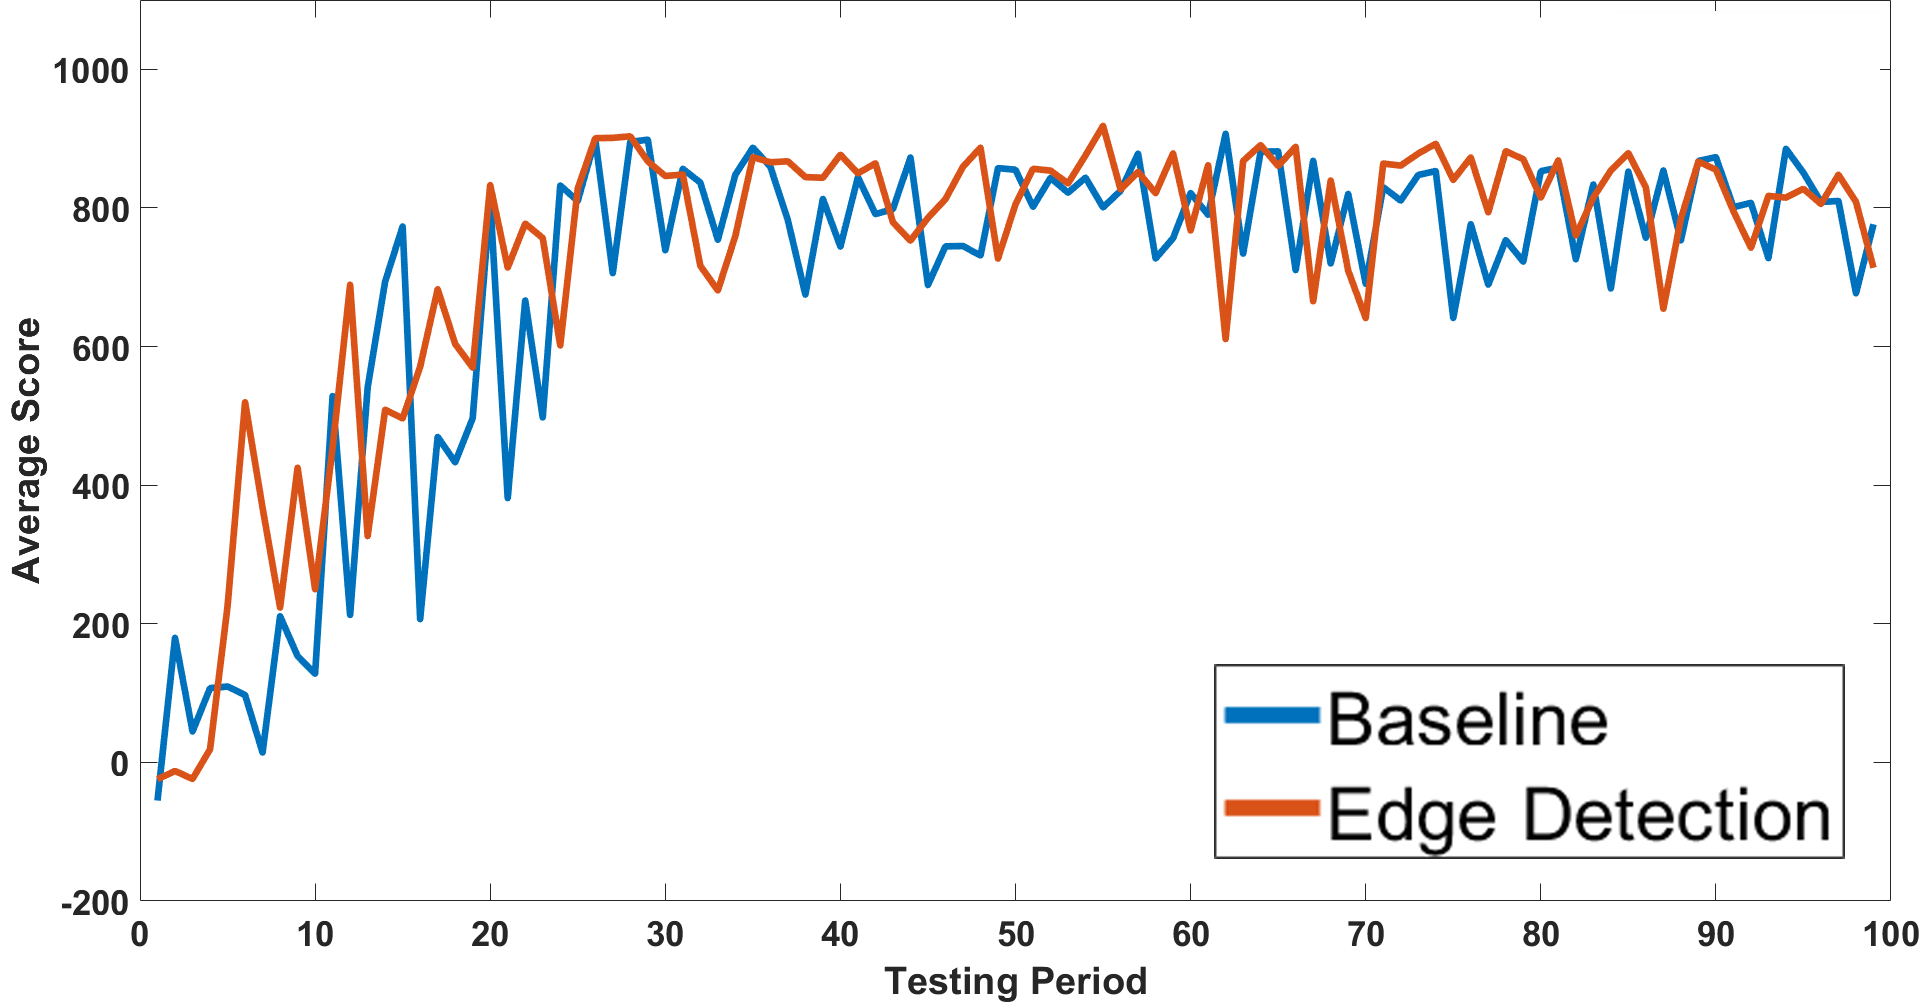
\includegraphics[width=.6\linewidth]{Graphics/edge_perf_score_large.png}
\caption{Average training score for edge detection}
\label{fig:test_edge}
\end{figure}

\newpage
\section{Grass Detection}
A common behavior exhibited by the agent is cutting corners as shown
in Figure \ref{fig:cut_corner}. 

\begin{figure}[h]
\centering
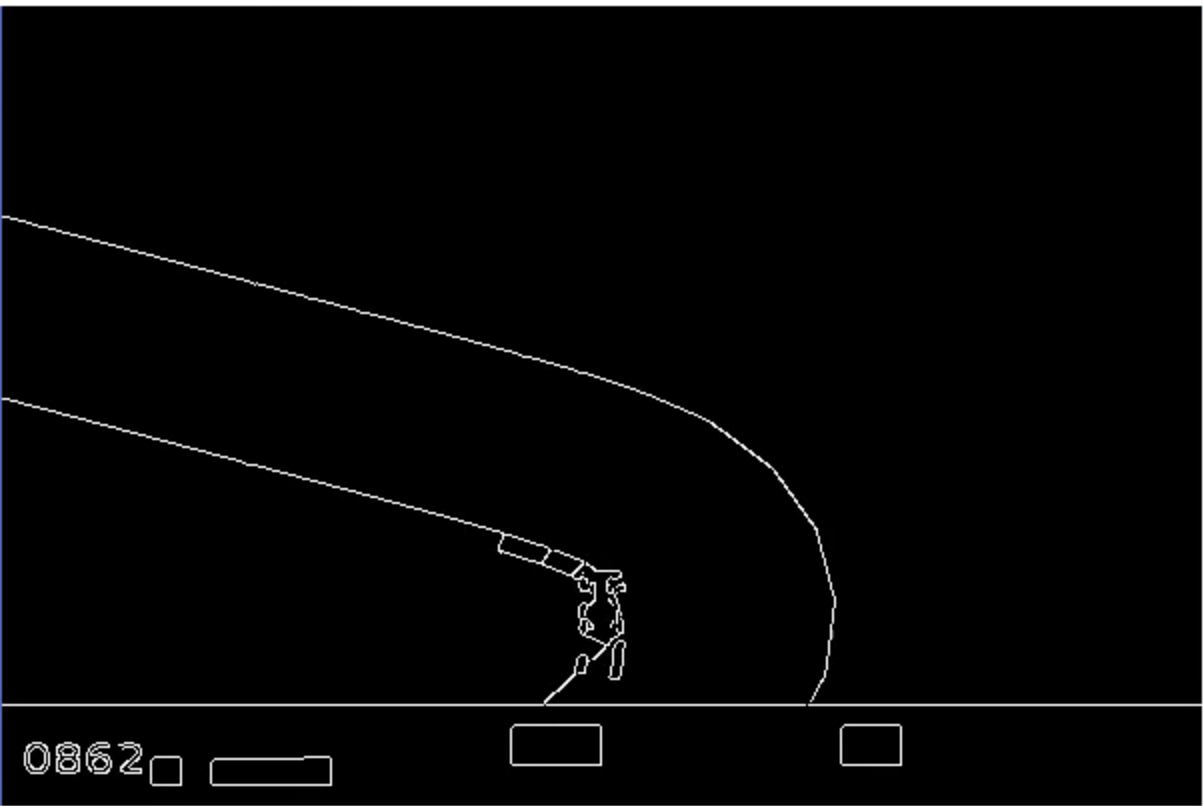
\includegraphics[width=0.6\textwidth]{Graphics/cut_corner.png}
\caption{Agent cuts corners}
\label{fig:cut_corner}
\end{figure}

Moreover, as commonly seen in professional race car driving, the 
car lingers along the right edge of the track to easily make left turns.
Consequently, when presented with a right turn, the agent has trouble
making it and often misses tiles. Both of these issues can be resolved
if the agent learns to stay out of the grass. While it is possible that
over time the agent will learn to stay out of the grass, the long training
time is undesirable. As such, we implemented a form of grass detection
so that the agent receives a negative reward while training to learn
to avoid the grass. The grass detection implementation is very simple: we 
simply crop a $13 \times 11$ rectangle around the car and count the
number of green pixels. If the number of green pixels is larger than 44, 
then we say the car is in the grass. 

\begin{figure}[]
\centering
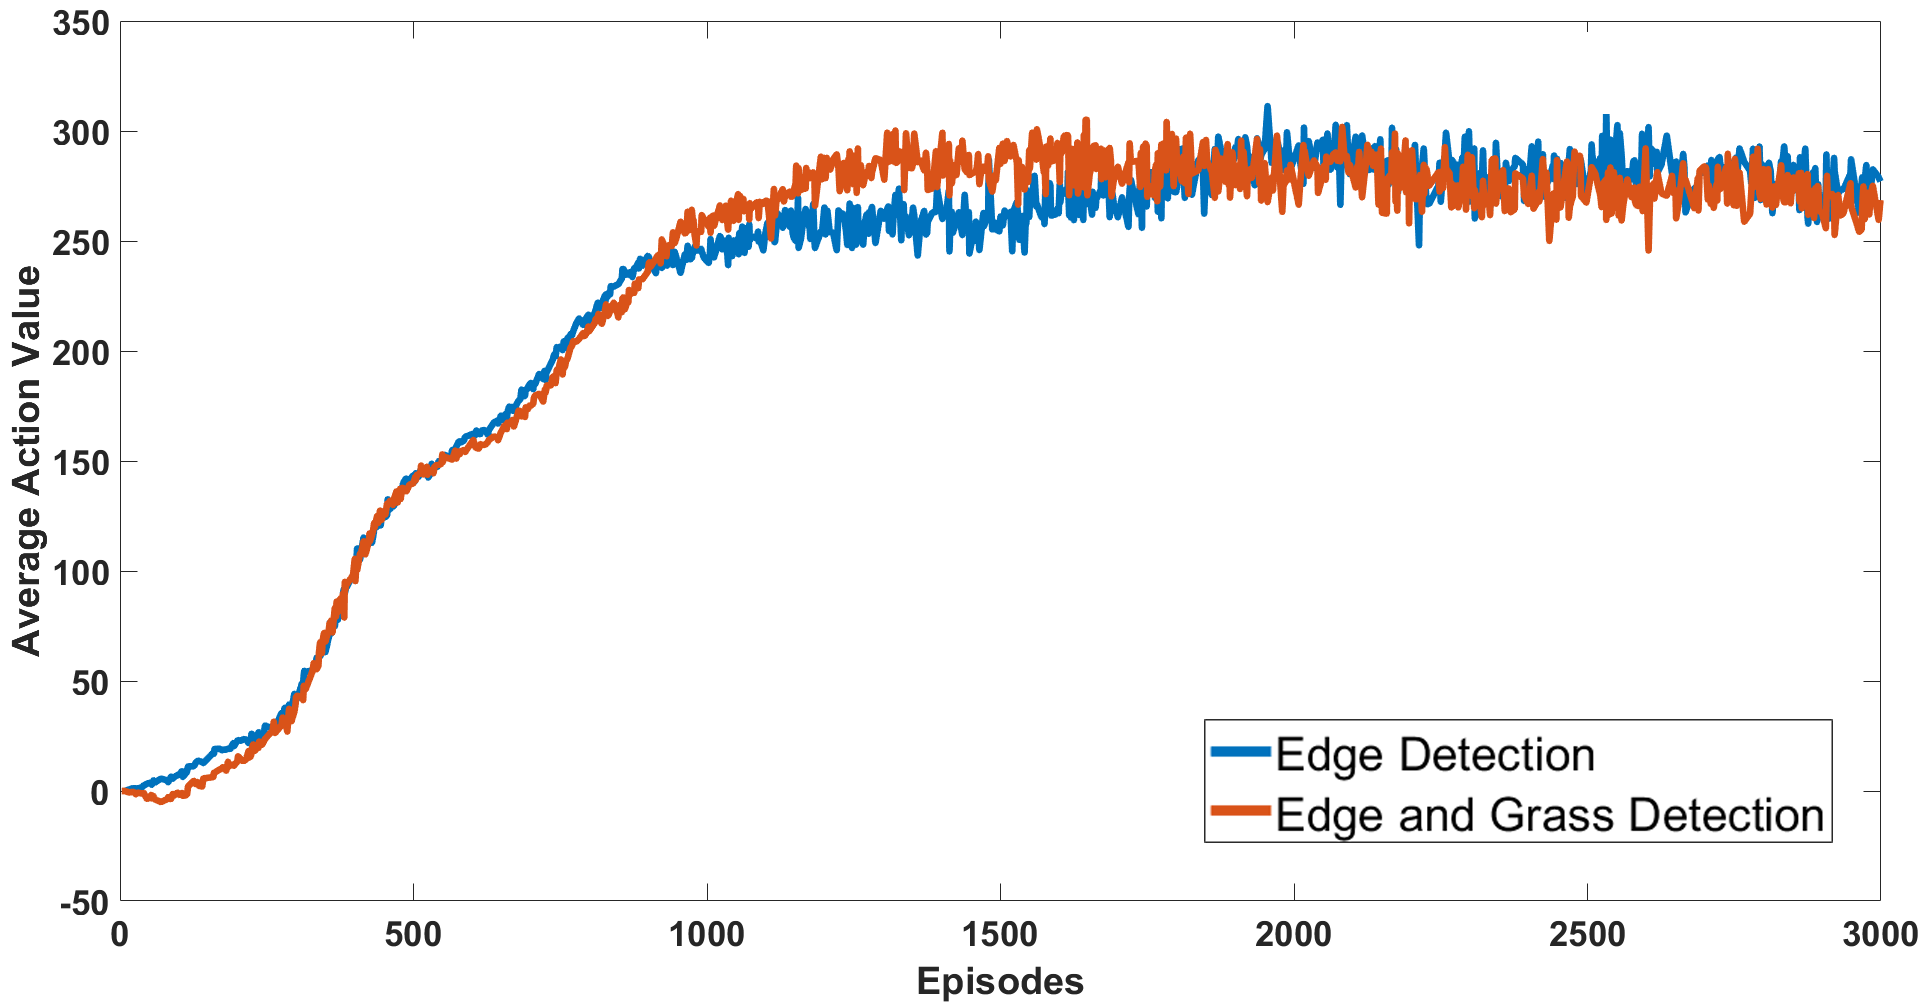
\includegraphics[width=.6\linewidth]{Graphics/grass_perf_q_large.png}
\caption{Average Q-value for grass detection}
\label{fig:grass_perf_q}
\end{figure}

\begin{figure}[h!]
\centering
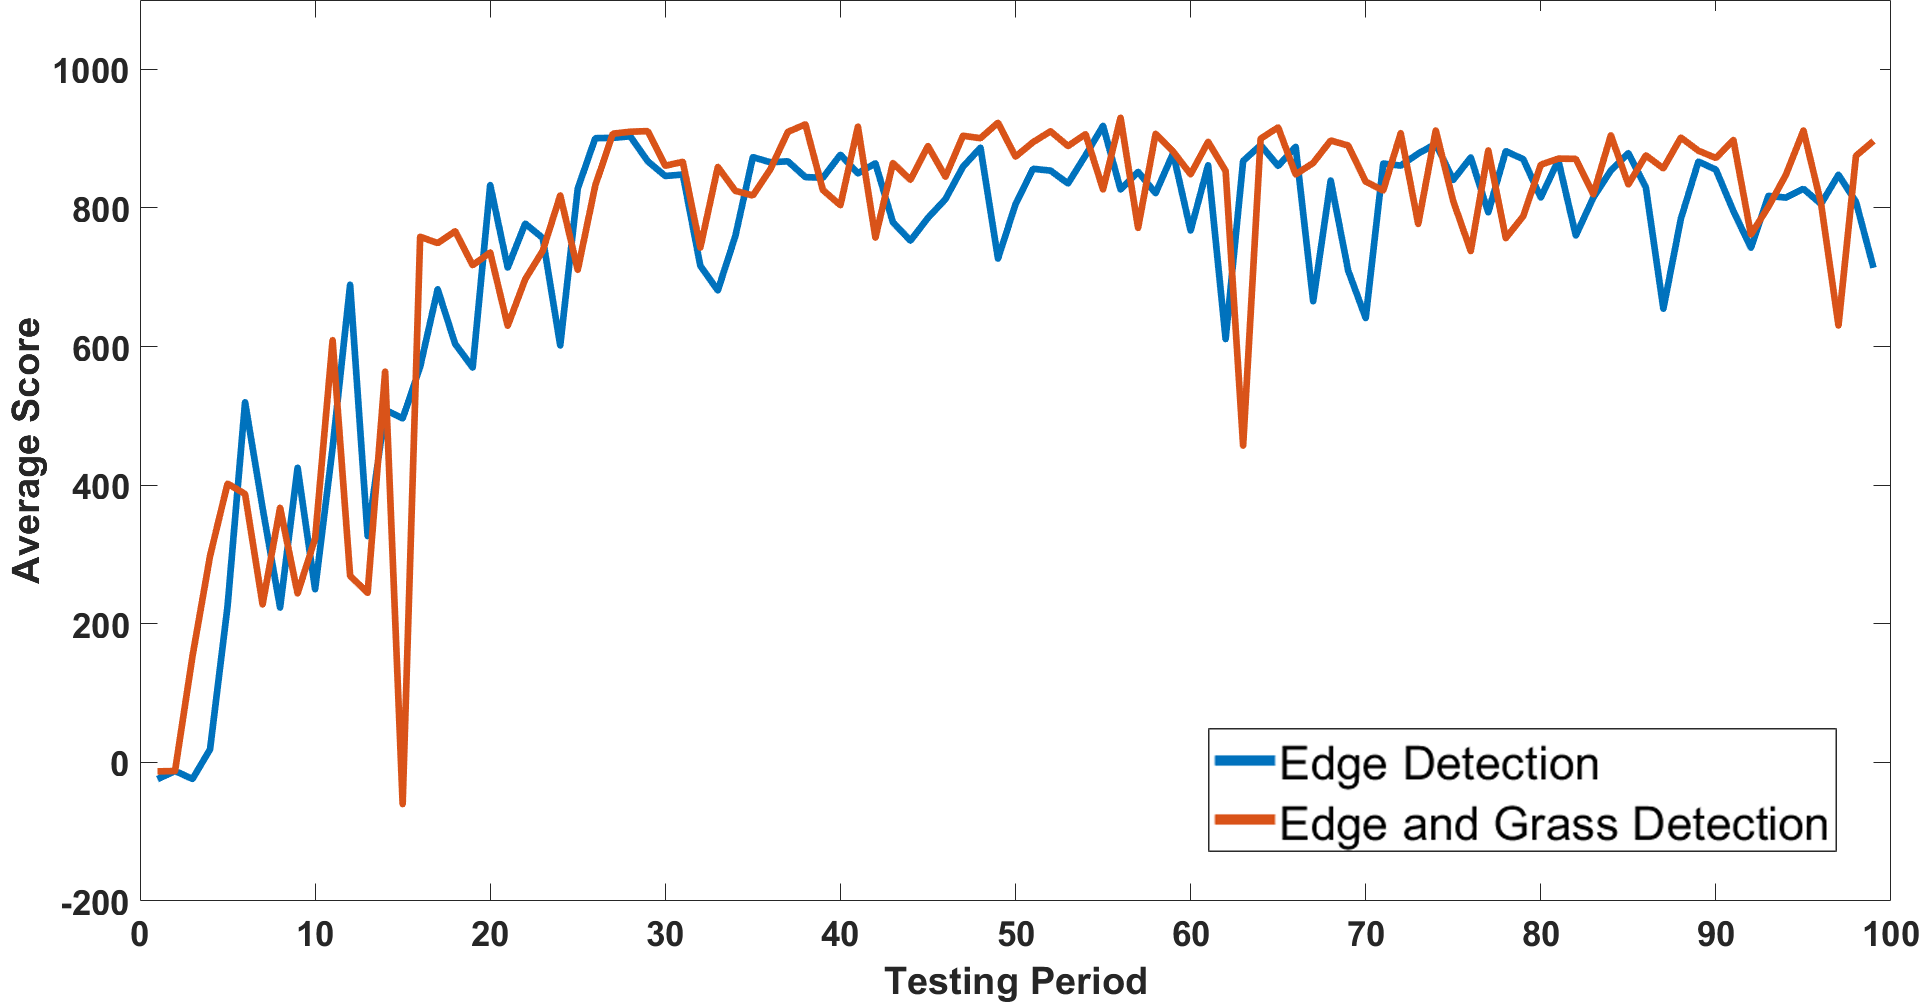
\includegraphics[width=.6\linewidth]{Graphics/grass_perf_score_large.png}
\caption{Average training score for grass detection}
\label{fig:grass_perf_score}
\end{figure}

As shown in Figure \ref{fig:grass_perf_q}, the average Q-value for
edge detection and edge with grass detection converge to the same values.
More importantly, as shown in Figure \ref{fig:grass_perf_score}, the training score
when using grass detection increases as compared to using edge detection
without grass detection. While both methods are able to exceed score of 
900, adding grass detection allows the agent to exceed the score more often
and reduces the number of times the car cuts corners. 

Our grass detection algorithm simply alters the reward function while 
training: it returns a score of -1 every time the car enters the grass.
In the context of real-world autonomous driving, grass detection can be 
interpreted as the auxiliary devices of the car. For example, the reward
given to the car while training can vary based on the distance between
the car and the sidewalk calculated with a radar.
Ultimately, 
incorporating grass detection into our algorithm while training, and
observing its performance on random tracks, suggests that 
such auxiliary data does not compromise the generalizability of our 
algorithm and improves its performance. 


\endinput





